\documentclass{beamer}
\usepackage[utf8]{inputenc}
\usepackage{graphicx}
\usepackage{url}

\author[Sowmya Vajjala]{Instructor: Sowmya Vajjala}


\title[LING 120]{LING 120: \\ Language and Computers}
\subtitle{Semester: Fall '17}

\date{01 November 2017}

\institute{Iowa State University, USA}

%%%%%%%%%%%%%%%%%%%%%%%%%%%

\begin{document}

\begin{frame}\titlepage
\end{frame}

\begin{frame}
\frametitle{Outline for today}
\begin{itemize}
\item Dialog Systems - Design (continued)
\item Evaluating Dialog Systems
\item Friday: Conclusion of dialog systems, and overview of Speech recognition.
\end{itemize}	
\end{frame}

\begin{frame}
\frametitle{Dialog Systems - What we discussed so far?}
\begin{itemize}
\item What are dialog systems?
\item Where are they useful?
\item What are the different kinds of dialog systems?
\item How are they created?
\item What are the aspects of dialogues these systems should take care of while chatting with a user?
\end{itemize}	
\end{frame}

\begin{frame}
\frametitle{Monday's exercise}
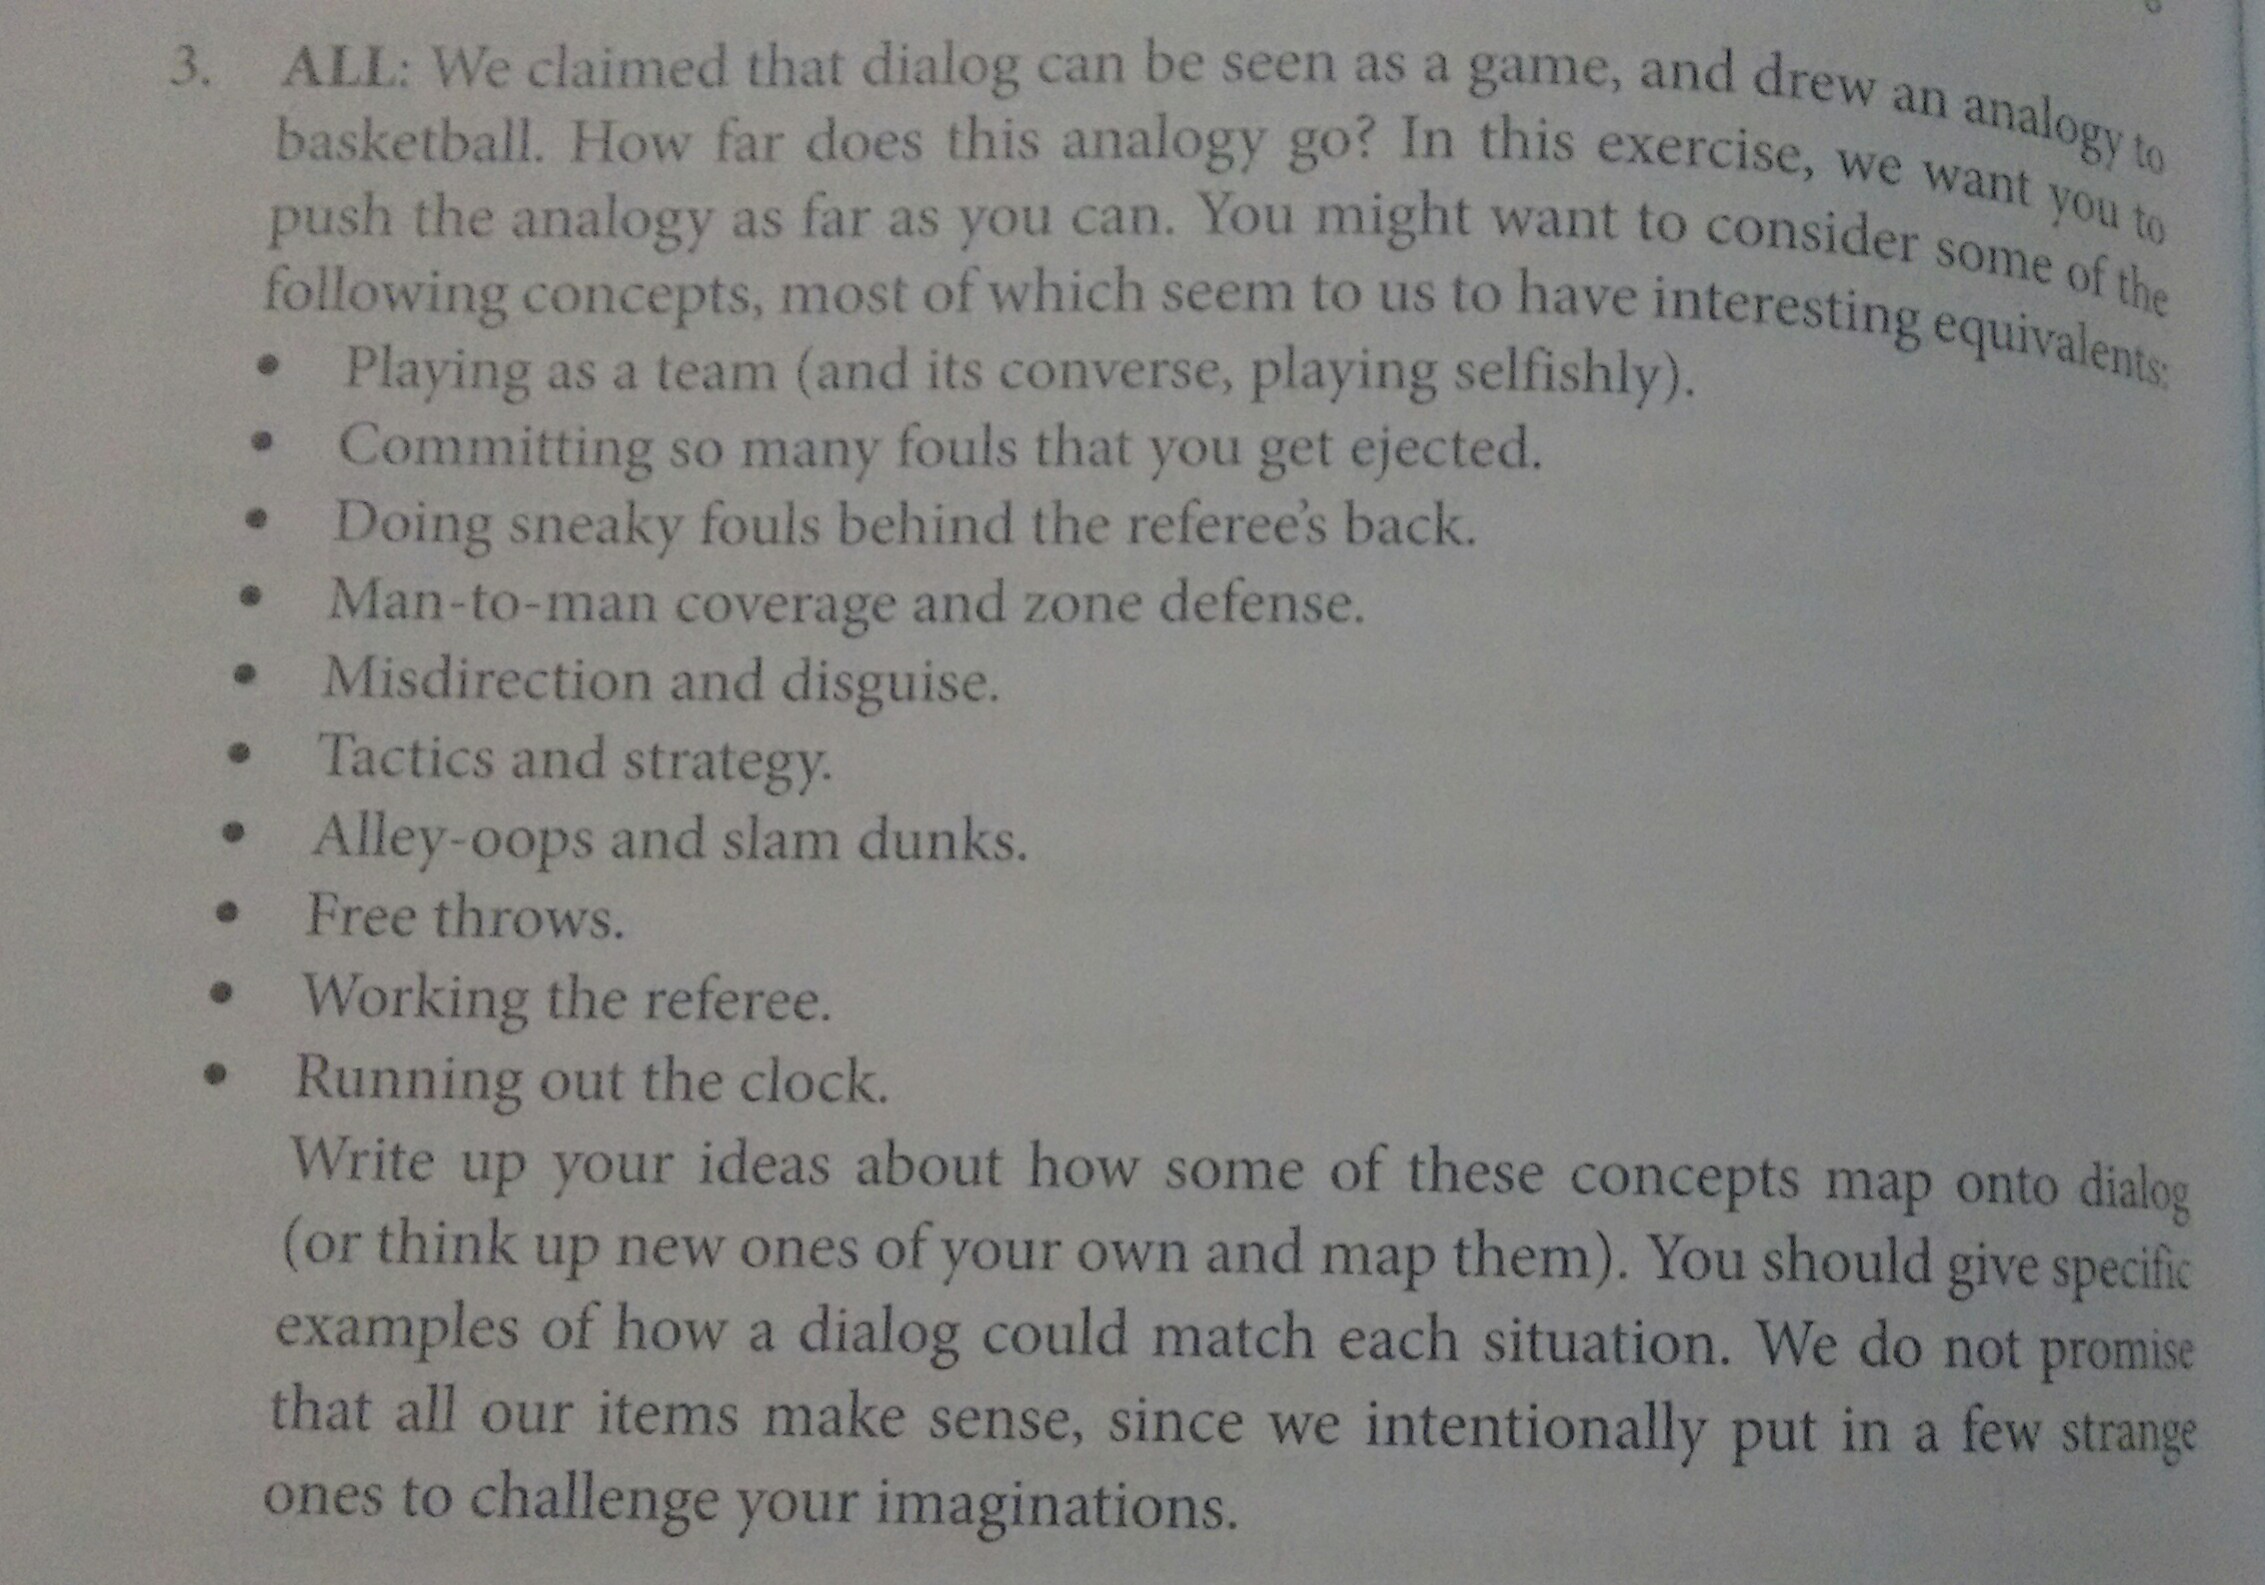
\includegraphics[width=0.9\textwidth]{question.jpg}
\end{frame}

\begin{frame}
\frametitle{Summary of Monday's responses}
\begin{itemize}
\item committing so many fouls you get ejected: giving rude responses until the other person quits the conversation.
\item running out the clock: rambling about random things
\item playing as a team: people should co-operate for smooth flow of conversation, lecture vs dialog
\item doing sneaky fouls behind the referees: backhanded compliments
\item mis-direction and disguise: misleading a conversation, lying with others in the conversation
\item tactics: staying away from touchy subjects
\end{itemize}	
\end{frame}

\begin{frame}
\frametitle{Recap Questions}
\begin{itemize}
\item How does Eliza work?  \pause
\item How can you add "Emotion" to Eliza, and make it show a variety of emotions such as happiness, sadness, anger etc? \pause
\item What is a frame based dialog system? \pause
\item How does a frame based dialog system differ from a chat bot? \pause
\item What is a Wizard of Oz simulation?
\end{itemize}	
\end{frame}

\begin{frame}
\frametitle{Another Example of Dialog System Development}
Interactions - \url{https://www.interactions.com/} - came with the idea of human-assisted dialog systems
\begin{itemize}
\item The idea is to have a human in the loop to improve the accuracy of dialog systems. 
\item i.e., not fully automated, but automation with human support 
\item (does that sound like a step backward? or a case of sensible implementation?)
\end{itemize}	
Adaptive Intelligence technology videos (\url{https://goo.gl/aTVFk3}, \url{https://goo.gl/LP9re7}) 
\end{frame}

\begin{frame}
\frametitle{Evaluation of Dialog Systems-1}
\begin{itemize}
\item According to you, how should these systems be evaluated objectively? \pause
\item Let us say, I am using a bot to assist customers do airline bookings. How do I know if the bot is doing well? \pause
\item How do we evaluate a multi-purpose system like Siri? \pause
\item Even before the bot starts interacting with customers, how can I evaluate it during development? \pause
\item As it turns out, this question has no easy answer!
\end{itemize}	
\end{frame}

\begin{frame}
\frametitle{Evaluation of Dialog Systems-2}
\begin{itemize}
\item Whether the dialog system manages to make a human feel he/she is chatting with another human \pause
\item Asking several human beta users to evaluate the system in terms of various features (speech recognition, response generation, language understanding, emotions, ability to converse etc) \pause
\item If we do not have users yet: Simulated dialog between two computers instead of a human and a computer \pause
\item More straight forward in some scenarios such as slot-filling ones in frame-based dialog systems - we can look for slot error rate. \pause
\item If possible response vocabulary is small, we can evaluate based on word-overlap between machine generated, and human generated response for the same question. 
\end{itemize}	
\end{frame}

\begin{frame}
\frametitle{Evaluation of Dialog Systems-Recent Advances}
Uses text classification, our previous topic!
\begin{itemize}
\item ADEM: Train a classifier on a set of responses in context, which are labeled as appropriate or inappropriate for the context by humans. You then use this classifier to evaluate responses of the dialog system. \pause
\item Adversarial Evaluation: Train a classifier to distinguish between human and machine generated responses first. If the dialog system successfully fools this evaluator, it is a good system.
\end{itemize}	
Note: This kind of work is very recent (above two examples are from July and September 2017 resp. !). 
\pause Something that is fresh-er (Today!): \url{https://www.wired.com/story/the-college-kids-doing-what-twitter-wont/}
\end{frame}

\begin{frame}
\frametitle{Attendance Exercise}
Go to the canvas forum, take a look at the uploaded file and work in groups of 2--3 people to answer the questions in the file. 
%http://www.nacloweb.org/resources/problems/2013/N2013-L.pdf 
\end{frame}

\end{document}
